\documentclass[tikz,border=10pt]{standalone}
\usepackage{pgfplots}
\usepackage{amsmath}
\pgfplotsset{compat=1.18}
\usetikzlibrary{arrows.meta, positioning, calc, fillbetween}

\definecolor{crimson}{RGB}{204, 0, 0}

\begin{document}
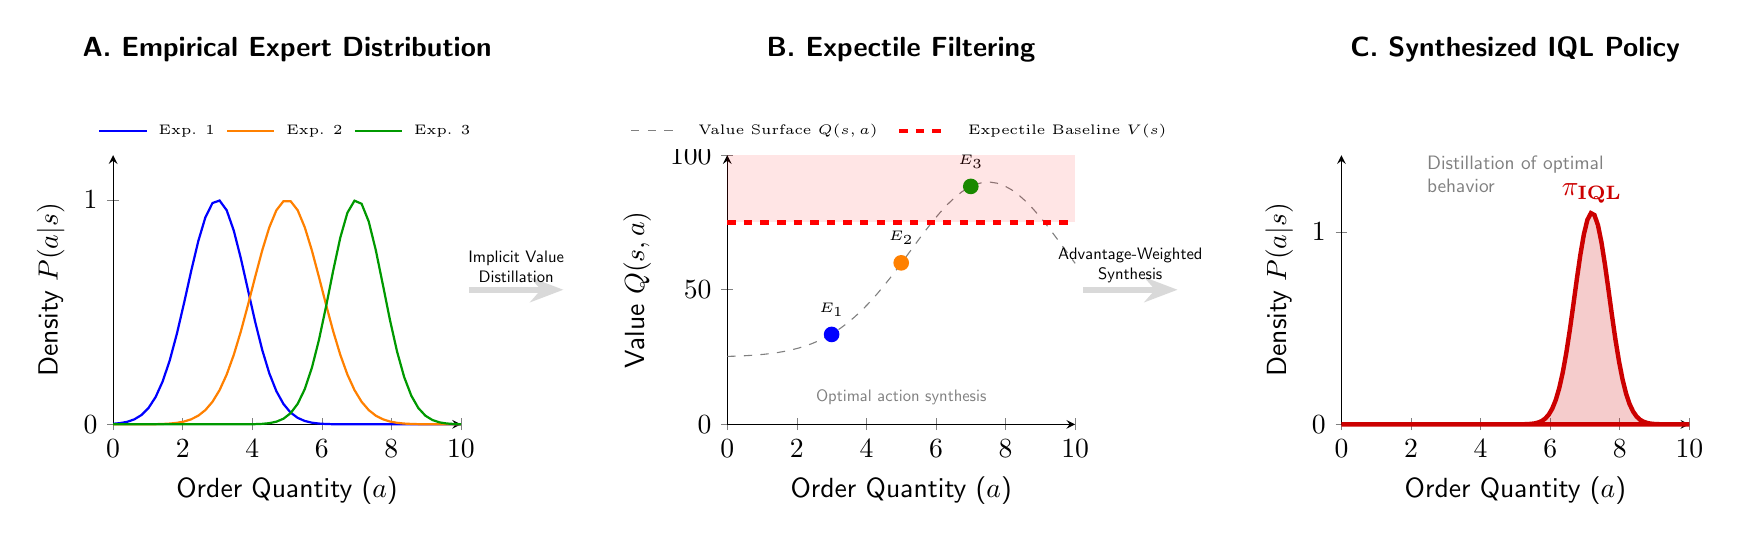
\begin{tikzpicture}[
    font=\sffamily,
    node distance=1cm,
    >=Stealth,
    expert1/.style={blue, thick},
    expert2/.style={orange, thick},
    expert3/.style={green!60!black, thick},
    iql/.style={crimson, ultra thick}
]

    % --- PANEL A: EXPERT MIXTURE ---
    \begin{scope}[local bounding box=panelA]
        \begin{axis}[
            width=6cm, height=5cm,
            at={(0,0)},
            axis y line=left,
            axis x line=bottom,
            xlabel={Order Quantity ($a$)},
            ylabel={Density $P(a|s)$},
            title={\textbf{A. Empirical Expert Distribution}},
            title style={at={(0.5,1.25)}, anchor=south},
            xmin=0, xmax=10,
            ymin=0, ymax=1.2,
            ytick={0, 1},
            name=axA,
            legend style={at={(0.5,1.02)}, anchor=south, font=\tiny, legend columns=3, draw=none, column sep=2pt},
            clip=false
        ]
            % Expert 1 (Low Stock Policy)
            \addplot[expert1, domain=0:10, samples=50] {exp(-(x-3)^2/1.5)};
            \addlegendentry{Exp. 1}
            
            \addplot[expert2, domain=0:10, samples=50] {exp(-(x-5)^2/2)};
            \addlegendentry{Exp. 2}
            
            \addplot[expert3, domain=0:10, samples=50] {exp(-(x-7)^2/1.2)};
            \addlegendentry{Exp. 3}
            
            \node[gray, scale=0.6, align=center] at (axis cs: 5, 1.3) {Heterogeneous historical logs};
        \end{axis}
    \end{scope}

    % --- ARROW 1 ---
    \draw[->, line width=2pt, gray!30] ($(axA.east) + (0.1,0)$ ) -- ($(axA.east) + (1.3,0)$ )
        node[midway, above, scale=0.6, text=black, align=center] {Implicit Value\\Distillation};

    % --- PANEL B: EXPECTILE FILTERING ---
    \begin{scope}[local bounding box=panelB, xshift=7.8cm]
        \begin{axis}[
            width=6cm, height=5cm,
            at={(0,0)},
            axis x line=bottom,
            axis y line=left,
            xlabel={Order Quantity ($a$)},
            ylabel={Value $Q(s,a)$},
            title={\textbf{B. Expectile Filtering}},
            title style={at={(0.5,1.25)}, anchor=south},
            xmin=0, xmax=10,
            ymin=0, ymax=100,
            ytick={0, 50, 100},
            name=axB,
            legend style={at={(0.5,1.02)}, anchor=south, font=\tiny, legend columns=2, draw=none, column sep=5pt},
            clip=false
        ]
            % Q-values (Conceptual landscape)
            \addplot[gray, dashed, domain=0:10, samples=50] {25 + 65*exp(-(x-7.5)^2/10)};
            \addlegendentry{Value Surface $Q(s,a)$}
            
            % Expert points (Aligned with the surface)
            \node[circle, fill=blue, inner sep=2pt, label=above:{\tiny $E_1$}] at (axis cs: 3, 33.4) {};
            \node[circle, fill=orange, inner sep=2pt, label=above:{\tiny $E_2$}] at (axis cs: 5, 60.0) {};
            \node[circle, fill=green!60!black, inner sep=2pt, label=above:{\tiny $E_3$}] at (axis cs: 7, 88.4) {};
            
            % Expectile Line V(s) - The "High Pass Filter"
            \addplot[red, ultra thick, dashed, domain=0:10] {75};
            \addlegendentry{Expectile Baseline $V(s)$}
            
            % Highlighted Advantage Region
            \fill[red, opacity=0.1] (axis cs: 0, 75) rectangle (axis cs: 10, 100);
            \node[gray, scale=0.6, align=center] at (axis cs: 5, 10) {Optimal action synthesis};
        \end{axis}
    \end{scope}

    % --- ARROW 2 ---
    \draw[->, line width=2pt, gray!30] ($(axB.east) + (0.1,0)$ ) -- ($(axB.east) + (1.3,0)$ )
        node[midway, above, scale=0.6, text=black, align=center] {Advantage-Weighted\\Synthesis};

    % --- PANEL C: SYNTHESIZED POLICY ---
    \begin{scope}[local bounding box=panelC, xshift=15.6cm]
        \begin{axis}[
            width=6cm, height=5cm,
            at={(0,0)},
            axis y line=left,
            axis x line=bottom,
            xlabel={Order Quantity ($a$)},
            ylabel={Density $P(a|s)$},
            title={\textbf{C. Synthesized IQL Policy}},
            title style={at={(0.5,1.25)}, anchor=south},
            xmin=0, xmax=10,
            ymin=0, ymax=1.4,
            ytick={0, 1},
            name=axC,
            clip=false
        ]
            % Synthesized Policy (Concentrated on high Q)
            \addplot[crimson, ultra thick, domain=0:10, samples=100, fill=crimson, fill opacity=0.2] 
                {1.1 * exp(-(x-7.2)^2/0.5)} \closedcycle;
            
            \node[crimson, font=\bfseries] at (axis cs: 7.2, 1.2) {$\pi_{\text{IQL}}$};
            \node[scale=0.7, gray, align=left] at (axis cs: 5, 1.3) {Distillation of optimal \\ behavior};
        \end{axis}
    \end{scope}

\end{tikzpicture}
\end{document}
